\documentclass[t]{beamer}
\usepackage{pgfpages}
\setbeameroption{show notes on second screen}

\setbeamertemplate{note page}{\insertnote}
\useoutertheme{infolines}

\setbeamertemplate{navigation symbols}{}

\usepackage[ruled,noline,noalgohanging]{algorithm2e}
\usepackage[english]{babel}
\usepackage[latin1]{inputenc}
\usepackage{times}
\usepackage[T1]{fontenc}
\usepackage{alltt}

\usepackage[makeroom]{cancel}

\usepackage{tikz}
\usetikzlibrary{calc,arrows,positioning,decorations.markings}
\usepackage{amsfonts}
\usepackage{amssymb}
\usepackage{amsmath}
\usepackage{wrapfig}
\usepackage{graphicx}
\usepackage{caption}
\usepackage{subcaption}
\usepackage{listings}
\usepackage{tabularx}
\usepackage{hyperref}
\captionsetup{compatibility=false}

\newtheorem{mylem}{Lemma}
\newtheorem{myeg}{Example}
\usepackage[ruled,noline,noalgohanging]{algorithm2e}

\usepackage[Euler]{upgreek}
\usepackage{xcolor,colortbl}

\title[]{Interactive Theorem Proving: Introduction}
\author[Formal Verification: 6CCS3VER]{Formal Verification: 6CCS3VER}

\tikzset{
  textnode/.style={},
  varnode2/.style={draw, outer sep=1pt},
  varnode2green/.style={draw,fill=green},
  varnode2red/.style={draw,fill=red},
  varnode2blue/.style={draw,fill=blue},
  varnode/.style={rectangle},
  varnodegreen/.style={rectangle,draw,fill=green},
  varnodered/.style={rectangle,draw,fill=red},
  varnodeblue/.style={rectangle,draw,fill=blue},
  varnodepurple/.style={rectangle,draw,fill=purple},
  varnodeyellow/.style={rectangle,draw,fill=yellow},
  varnodeempty/.style={inner sep=0pt,fill},
  line/.style={=stealth,thick,fill=red},
  matchededge/.style={>=stealth,thick,fill=black},
  unmatchededge/.style={>=stealth,thick,fill=blue},
  arrow/.style={=>stealth,thick}
}


\setbeamertemplate{itemize/enumerate body begin}{\large}
\setbeamertemplate{itemize/enumerate subbody begin}{\large}
\setbeamertemplate{itemize/enumerate subsubbody begin}{\large}
\setbeamertemplate{itemize/enumerate subsubsubbody begin}{\large}

\usepackage{enumitem}
\setlistdepth{20}
%% \renewlist{itemize}{itemize}{20}
%% \renewlist{enumerate}{enumerate}{20}
%% \setlist[itemize]{label=$\cdot$}
\setlist[itemize,1]{label=\textbullet}
\setlist[itemize,2]{label=--}
\setlist[itemize,3]{label=*}
\setlist[itemize,4]{label=$\cdot$}
\setlist[itemize,5]{label=$->$}
\setlist[itemize,6]{label=$->$}
\setlist[itemize,7]{label=$->$}
\setlist[itemize,8]{label=$->$}

% The main document
\date{}
\begin{document}


\begin{frame}[t]
  \titlepage

\note<1->{
\scriptsize
\begin{itemize}
\item Hello everyone, this is Mohammad Abdulaziz, a lecturer at the dept of informatics
\item I do research in interactive theorem proving and its applications to making sure that AI systems and algorithms are safe (I will say a bit more about that)
\item I will be teaching you three lectures on interactive theorem proving, an important technique used for formal verification and other things
\end{itemize}}

\end{frame}

\begin{frame}{This Video}
\newcommand{\intro}{1}
\only<\intro>{
\begin{itemize}
  \item What is interactive theorem proving?
  \item What are we doing over the next three lectures?
  \item What do I expect you to already know?
  \item Some Organisational notes
\end{itemize}
}

\note<\intro->{
\scriptsize
In this video I will
\begin{itemize}
  \item Introduce you to interactive theorem proving, the main idea, and motivate why I think it is an interesting technology to learn about
  \item I will then discuss briefly what are we doing over the next three lectures, which talk about ITPing, including the learning objectives
  \item I will also briefly discuss what concepts and techniques I expect you to already know from previous modules, although I will briefly introduce the different concepts throughout the lectures
  \item I will discuss some organisational notes regarding these next lectures and the coursework
 \end{itemize}
}
\end{frame}

\begin{frame}{What is ITP'ing?}
\newcommand{\syllogism}{1}
\newcommand{\formalproof}{2}
\newcommand{\axioms}{3}
\newcommand{\whyformal}{4}
\newcommand{\verybigproofs}{5}
\newcommand{\computerbasedformalproofs}{6}
\newcommand{\computerbasedformalproofseg}{7}
\newcommand{\formalproofmaths}{8}
\newcommand{\formalproofCS}{9}
\newcommand{\formalproofmywork}{10}

\note<\syllogism>{
\tiny
  \begin{itemize}
  \item Before I talk about interactive theorem proving I want to recapitulate with you the concept of formal proof
  \item Recall with me the following Aristotlian syllogism
    \begin{itemize}
    \item All men are mortal (Assume)
    \item Aristotle is a man (Assume)
    \item Aristotle is mortal (from 1, 2, and modus-ponens)
    \end{itemize}
  \item I hope we all agree that this is an unambiguously correct proof
  \end{itemize}
}

\only<\syllogism>{
  Formal proofs:
  \begin{itemize}
  \item Recall with me the following Aristotlian syllogism
    \begin{itemize}
    \item 1: All men are mortal (Assume)
    \item 2: Aristotle is a man (Assume)
    \item 3: Aristotle is mortal (from 1, 2, and modus-ponens)
    \end{itemize}
  \item Modus-ponens: if a implies b and a holds, then b holds
  \item I hope we all agree that this is an unambiguously correct proof
  \end{itemize}
}

\note<\formalproof>{
\tiny
  \begin{itemize}
  \item Our goal is to construct formal proofs of correctness for mathematical theorems and for algorithms/systems
  \item This is because formal proofs are the closest thing to objectively and unambiguously correct proofs:
    \begin{itemize}
    \item By that I maen, definitions and theorem statements whose meaning and well-formedness are unambiguosly correct
    \item And also proof that are unambiguously correct
    \item This is to be done wrt precisely and concisely stated axioms that indicate 
          what are correct reasoning or proof steps, and what is the meaning of different statements or claims
    \end{itemize}
  \end{itemize}
}

\only<\formalproof>{
  \begin{itemize}
  \item Our objective: construct formal proofs
  \item Unambiguous, correct proofs:
    \begin{itemize}
    \item Definitions' and theorem statements' meaning and well-formedness
    \item Proof correctness
    \end{itemize}
  \item All of that wrt precisely and concisely stated axioms
  \end{itemize}
}

\note<\axioms>{
  \tiny
  \begin{itemize}
  \item Proofs and definitions are written in formal language whose meaning is defined by set of axioms, e.g.
    \begin{itemize}
    \item Linear temporal logic axioms (recall from week 3 lecture)
    \item or Zermelo-Fraenkel set theory that are capable of representing any mathematical statement or thm, and they are more general than LTL. Some of its axioms are as follows
      \begin{itemize}
        \item Extensionality: {\small $\forall s,t.\; (\forall x.\; x\in s \leftrightarrow x\in t) \rightarrow s = t$}
        \item Regularity: {\small $\forall s.\; s\neq\emptyset \rightarrow \exists t.\; t\in s \wedge t\cap s =\emptyset$}
        \item Schema: {\small $\forall s,x_1,\dots,x_n.\exists t.\; \forall y.\; y\in t \leftrightarrow (y\in s \wedge \phi(s,x_1,\dots,x_n,y))$}
        \item \dots
      \end{itemize}
    \item there is also Type theory
    \item Peano Arithmetic
    \item First-order logic
    \item and Higher-order logic (HOL), which is the logical system of the theorem prover we use here
    \end{itemize}
  \end{itemize}
}

\only<\axioms>{
  \begin{itemize}
  \item Proofs and definitions are written in a formal language
  \item Meaning is defined by set of axioms, e.g.
    \begin{itemize}
    \item Linear temporal logic axioms (recall from week 3 lecture)
    \item More general: Zermelo-Fraenkel set theory:
      \begin{itemize}
        \item Extensionality: {\small $\forall s,t.\; (\forall x.\; x\in s \leftrightarrow x\in t) \rightarrow s = t$}
        \item Regularity: {\small $\forall s.\; s\neq\emptyset \rightarrow \exists t.\; t\in s \wedge t\cap s =\emptyset$}
        \item Schema: {\small $\forall s,x_1,\dots,x_n.\exists t.\; \forall y.\; y\in t \leftrightarrow (y\in s \wedge \phi(s,x_1,\dots,x_n,y))$}
        \item \dots
      \end{itemize}
    \item Others formalisms
      \begin{itemize}
      \item Type theory, Peano Arithmetic, First-order logic, and \textcolor{red}{Higher-order logic (HOL)}
      \end{itemize}
    \end{itemize}
  \end{itemize}
}

\note<\whyformal>{
\tiny
  \begin{itemize}
  \item The initial reason to bother with formal proofs, which is still very relevant (later on that), is to ``formalise'' mathematics, which was more of an intellectual curiosity
    \begin{itemize}
    \item Some of the earliest trials to get formal proofs, i.e.\ to fully specify the axioms and show how every step in the proof follows from those axioms, are Euclid's elements (~300 B.C.) and principia mathematica [Russel and Whitehead 1910] 
    \end{itemize}
  \end{itemize}
}

\only<\whyformal>{
  \begin{itemize}
  \item Why formal proofs?
  \item Initially to ``formalise'' mathematics
    \begin{itemize}
    \item E.g.\ Euclid's elements (~300 B.C.) and principia mathematica [Russel and Whitehead 1910] 
    \end{itemize}
  \end{itemize}
}

\note<\verybigproofs>{
\tiny
  \begin{itemize}
  \item A challenge, however, to that way of doing mathematics is size of a formal proof
    \begin{itemize}
    \item An example from Russel and Whitehead's attempt is shown on the slide, where in their book on formal mathematics they were able to prove that 1+1=2 after 173 pages of definitions and proofs
    \item Because of that, it was seen as unrealistic for any non-trivial proofs, due to size and tedium, and 
    \item it never took-off, except as a theoretical idea
    \end{itemize}
    %% \begin{center}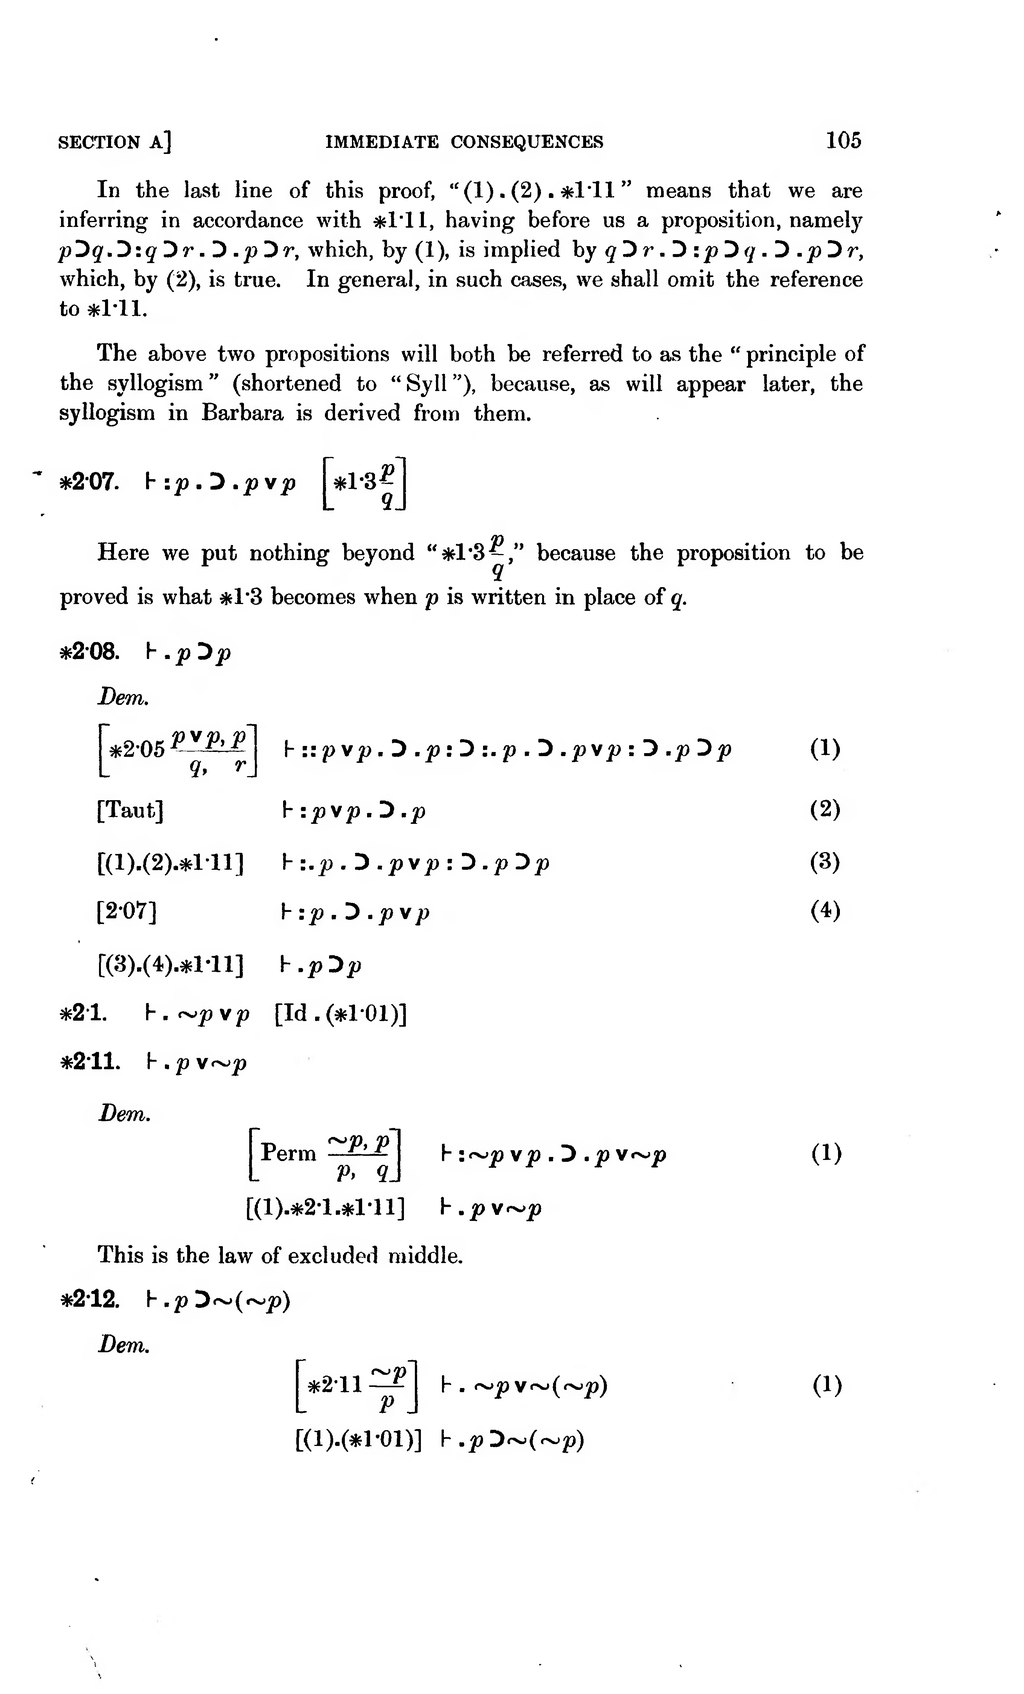
\includegraphics[height=\textheight]{ruseel.jpg}\end{center}
    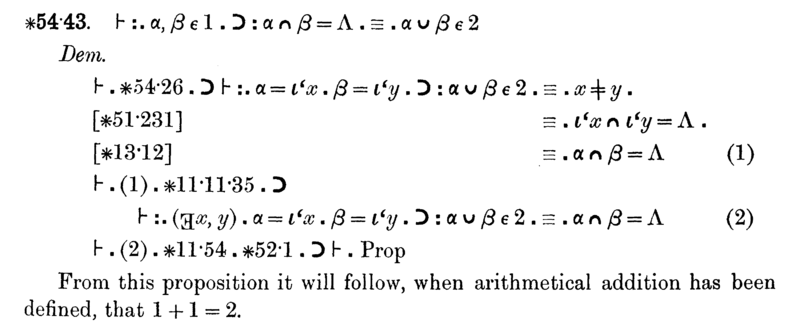
\includegraphics[width=\textwidth]{Principia-Mathematica-1.png}
  \end{itemize}
}

\only<\verybigproofs>{
  \begin{itemize}
  \item Challenge: is the size of a formal proof
    \begin{itemize}
    \item Russel and Whitehead prove that 1+1=2 after 173 pages
    \end{itemize}
    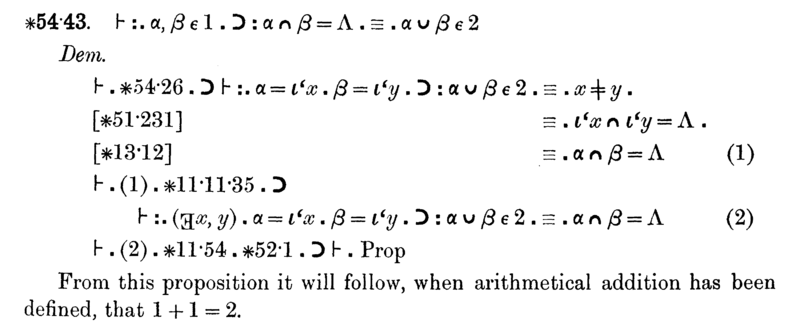
\includegraphics[width=\textwidth]{Principia-Mathematica-1.png}
  \item Unrealistic for non-trivial proofs, due to size and tedium
  \item Never took-off, except as a theoretical idea
    %% \begin{center}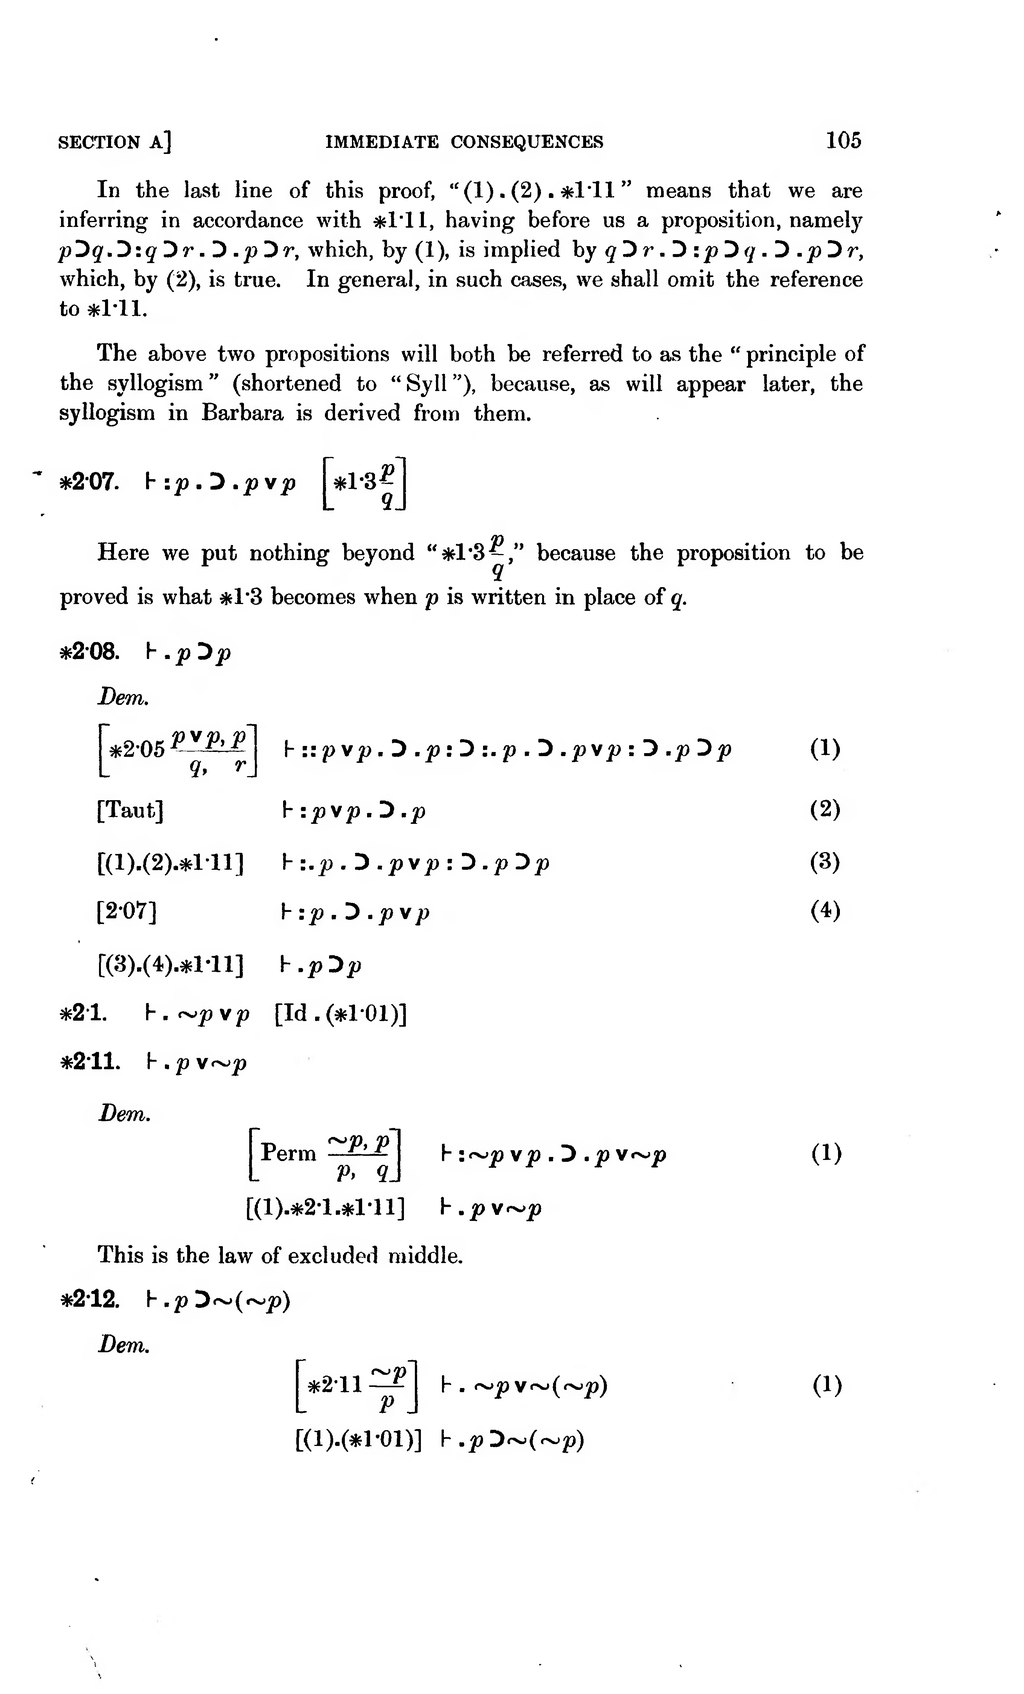
\includegraphics[height=\textheight]{ruseel.jpg}\end{center}
  \end{itemize}
}


\note<\computerbasedformalproofs>{
  \tiny
  \begin{itemize}
  \item A turning point happened to formal mathematics with the advent of digital computers
  \item Since computers can be very effective at generating and checking these very long formal proofs
    \begin{itemize}
    \item One approach to computer-based formal maths is that of automated theorem provers, where the computer generates a formal proof and checks that it is correct according to the logic's axioms.
    \item Examples of this approach are model-checkers, with which you must be very well acquainted, and also SAT-solvers, which you will learn about during the last lecture, and also first-order logic ATPs
      \begin{itemize}
      \item model-checkers
      \item SAT-solvers
      \item first-order logic automatic theorem provers
      \end{itemize}
    \item Although these automated methods have the advantage that they are push-button, they have the problem that they does not scale to bigger or more conceptually complicated mathematics
    \item Fundamental reasons for that are G�del's incompleteness theorem, undecidability of the halting problem
    \item Practical implications include for instance that one cannot prove that an algorithm is correct for any input automatically for any given algorithm, or to automatically prove different mathematical theorems about primes, etc.
    \item However, a practically very successful compromise is the approach of interactive theorem provers (ITPs) like
      \begin{itemize}
      \item Isabelle/HOL [Nipkow et al.\ 2002], HOL4 [Slind and Norrish 2008], Coq [Bertot and Casteran], Lean
      \end{itemize}
    \item ITPs are mechanised formal mathematical systems
    \item in which one specifies definitions, statements, and proofs in a formal language
    \item and the ITP makes sure that the proof only follows from a specific set of axioms
    \item in our case, we use the ITP Isabelle/HOL
    \item An example proof using that system is on the slide, where a proof of the fact that sqrt 2 is irrational is presented.
    \item As shown here, the user enters high-level steps of the proof, and the ITP fills in the details to make sure that the proof is valid down to the level of logical axioms
    \end{itemize}
  \end{itemize}

}

\only<\computerbasedformalproofs>{

  \begin{itemize}
  \item Machines can check proofs, and generate them
    \begin{itemize}
    \item Automated theorem provers 
      \begin{itemize}
      \item model-checkers
      \item SAT-solvers
      \item first-order logic automatic theorem provers
      \end{itemize}
    \item Problem: does not scale 
    \item Interactive theorem provers (ITPs)
      \begin{itemize}
      \item e.g. Isabelle/HOL [Nipkow et al. 2002], HOL4 [Slind and Norrish 2008], Coq [Bertot and Casteran], Lean [de Moura]
      \end{itemize}
    \end{itemize}

  \end{itemize}
}

\note<\computerbasedformalproofseg>{
  \tiny
  \begin{itemize}
    \item ITPs are mechanised formal mathematical systems
    \item in which one specifies definitions, statements, and proofs in a formal language
    \item and the ITP makes sure that the proof only follows from a specific set of axioms
    \item in our case, we use the ITP Isabelle/HOL
    \item An example proof using that system is on the slide, where a proof of the fact that sqrt 2 is irrational is presented.
    \item As shown here, the user enters high-level steps of the proof, and the ITP fills in the details to make sure that the proof is valid down to the level of logical axioms
  \end{itemize}

}

\only<\computerbasedformalproofseg>{
  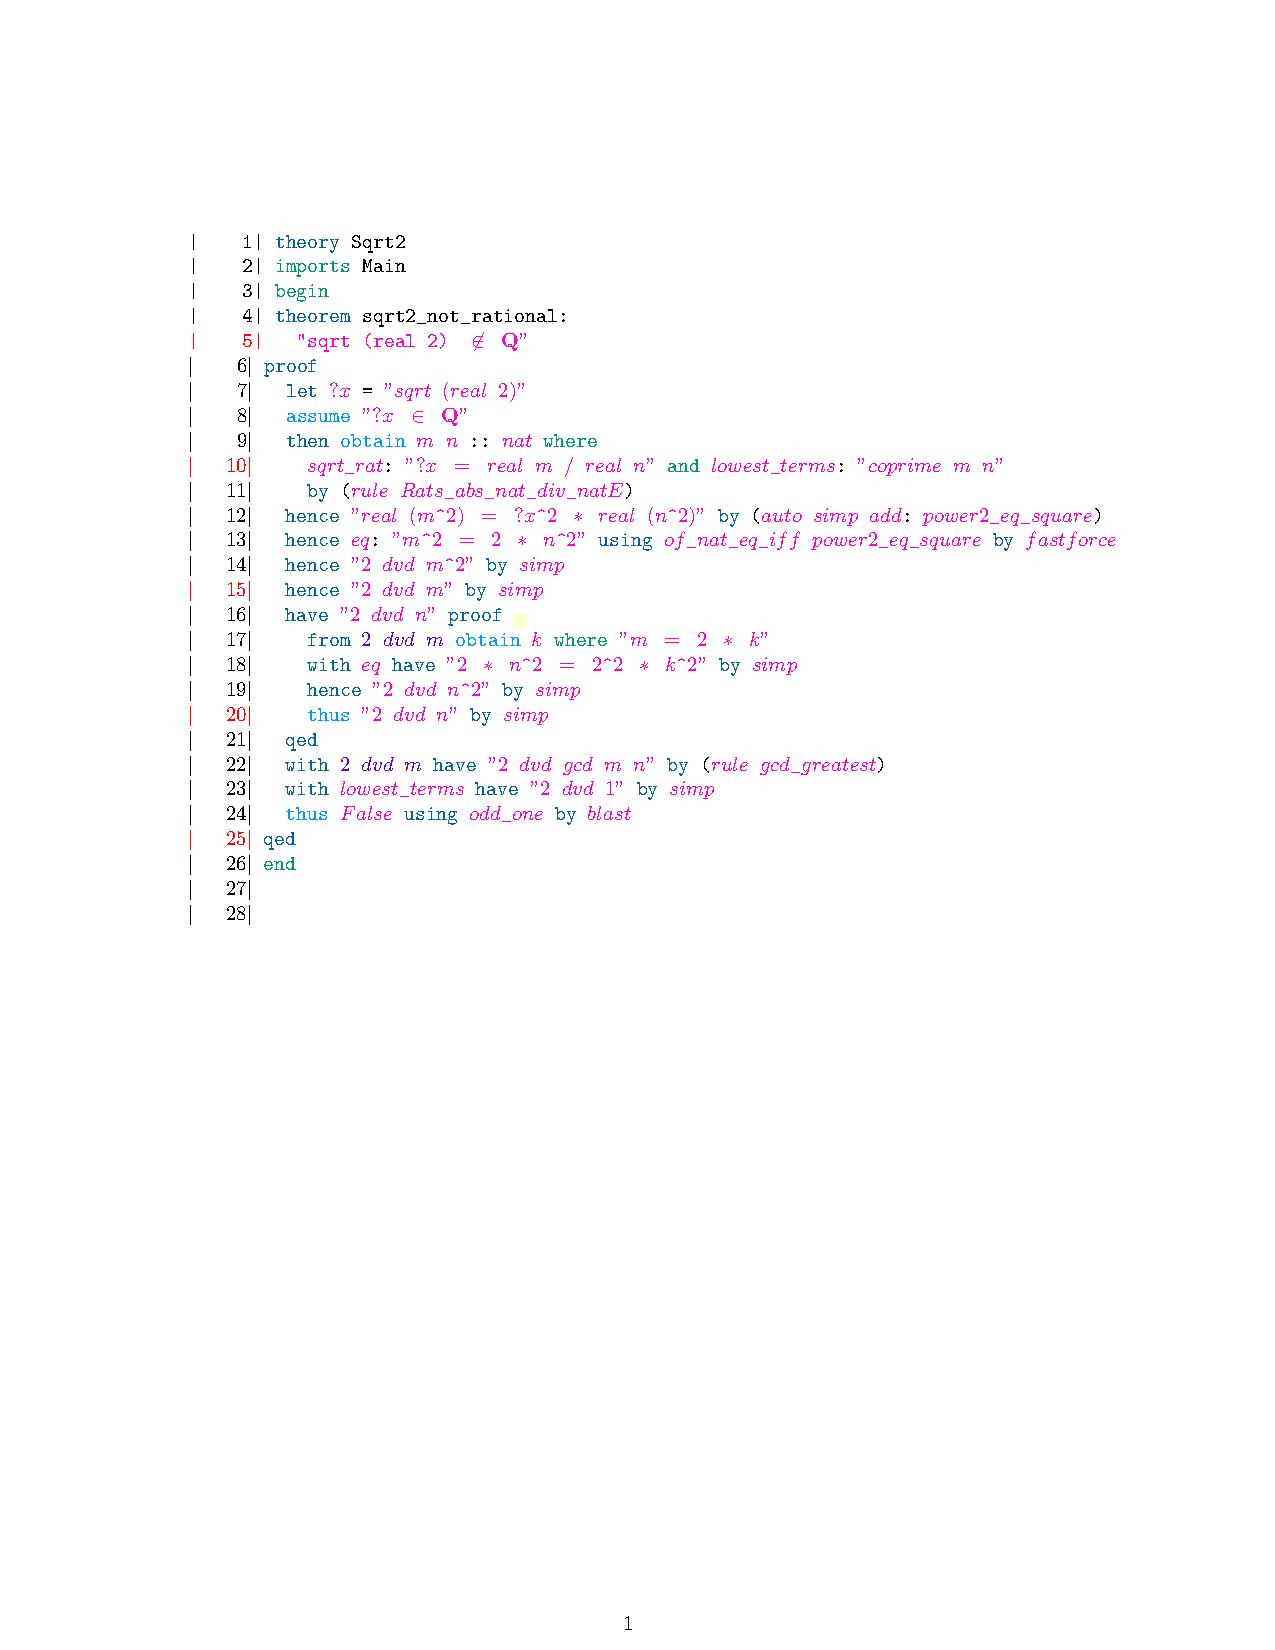
\includegraphics[width=\textwidth,clip=,trim=80 0 0 100]{Sqrt2Test.pdf}
}

\note<\formalproofmaths>{
  \tiny
  \begin{itemize}
  \item ITPs are more successful for practising formal proof, in both maths and computer science
  \item Notable applications to formal mathematics
    \begin{itemize}
    \item four-colour theorem [Gonthier 2007]
    \item odd-order theorem [Gonthier et al. 2013]
    \item Kepler's conjecture [Hales et al. 2015]
    \item There is also a list of the `` most interesting'' 100 theorems, which keeps tracks of which theorems were formally proved
    \item Also recently proof assistants were used to formally prove a \href{https://www.quantamagazine.org/lean-computer-program-confirms-peter-scholze-proof-20210728/}{theorem} whose correctness was doubted in the area of number theory
    \end{itemize}
  \end{itemize}
}

\only<\formalproofmaths>{
  \begin{itemize}
  \item Notable applications in formal mathematics
    \begin{itemize}
    \item four-colour theorem [Gonthier 2007]
    \item odd-order theorem [Gonthier et al. 2013]
    \item Kepler's conjecture [Hales et al. 2015]
    \item 98\% of the `` most interesting'' \href{https://www.cs.ru.nl/~freek/100/}{\textcolor{red}{100 theorems}}
    \item  \href{https://www.quantamagazine.org/lean-computer-program-confirms-peter-scholze-proof-20210728/}{\textcolor{red}{The Liquid-Tensor Experiment}}
    \end{itemize}
  \end{itemize}
}

\note<\formalproofCS>{
  In CS formal proof is used for \emph{formal verification}:
    \begin{itemize}
    \item A system and its desired properties are specified in a formal language
    \end{itemize}
  Notable application in CS:
    \begin{itemize}
    \item To get reliable implementations of complicated algorithms and software. This includes
      \begin{itemize}
      \item SeL4: Linux Kernel [Klein et al. 2009]
      \item CompCert: compiler for C [Leroy 2009]
      \item CakeML: compiler for a flavour of ML [Kumar et al. 2014]
      %\item verified certificate checkers [Mehlhorn et al. 2014, Abdulaziz and Lammich 2018, Lammich 2018, Wimmer 2019]
      \item and even a fully verified model-checker [Esparza et al. 2013], i.e.\ if it tells a specification has no counter examples, then it definitely doesn't
      \item SAT-solver [Blanchette et al. 2018, Fleury 2019]
      \end{itemize}
    \end{itemize}  
  It is also being more and more adopted by industry in the area of ciritical software formal verificaiton, e.g.\ cryptographic software in apple, many parts of AWS infrastructure, as well as hardware and firmware in Arm and Intel

  I have added some links to the job openings related to theorem proving at these companies, which of course will change with time
}


\only<\formalproofCS>{
\begin{itemize}
  \item In CS formal proof is used for \emph{formal verification}:
    \begin{itemize}
    \item A system and its desired properties are specified in a formal language
    \end{itemize}
  \item Notable application in CS:
    \begin{itemize}
    \item To get reliable implementations
      \begin{itemize}
      \item SeL4: Linux Kernel [Klein et al. 2009]
      \item CompCert: compiler for C [Leroy 2009]
      \item CakeML: compiler for a flavour of ML [Kumar et al. 2014]
      %\item verified certificate checkers [Mehlhorn et al. 2014, Abdulaziz and Lammich 2018, Lammich 2018, Wimmer 2019]
      \item model-checker [Esparza et al. 2013]
      \item SAT-solver [Blanchette et al. 2018]
      \end{itemize}
    \end{itemize}
  \item Adopted by industry:
    \begin{itemize}
    \item \href{https://jobs.intel.com/search-jobs?k=theorem+proving&l=&orgIds=599}{\textcolor{red}{Intel}}, \href{https://careers.arm.com/search-jobs/theorem\%20proving?orgIds=34601&kt=1}{\textcolor{red}{Arm}}, \href{https://www.amazon.jobs/en/search?offset=0&result_limit=10&sort=relevant&distanceType=Mi&radius=24km&latitude=&longitude=&loc_group_id=&loc_query=&base_query=theorem\%20proving&city=&country=&region=&county=&query_options=&}{\textcolor{red}{AWS}}, \href{https://jobs.apple.com/en-gb/search?page=5&sort=relevance&search=theorem\%20proving}{\textcolor{red}{Apple}}
    \end{itemize} 
  \end{itemize}  
}

\note<\formalproofmywork>{
\begin{itemize}
  \item Finally, I would like to note that a lot of my own work is in the application of ITPs to
  \begin{itemize}
    \item the verification of algorithms and software in the areas of automated planning, solving MDPs, ML, and reinforcement learning
    \item formalisation of mathematics, especially complexity theory and the theory of combinatorial optimisation
  \end{itemize} 
  \item If that interests any of you for a final year project, let's have a chat!
\end{itemize}
}


\only<\formalproofmywork>{
\begin{itemize}
  \item Some of my own \href{https://home.in.tum.de/~mansour/cv-and-website/website/index.html}{\textcolor{red}{research}}:
  \begin{itemize}
    \item verification of AI and ML
    \item formalisation of mathematics, esp.\ complexity theory and combinatorial optimisation
  \end{itemize} 
  \item If that interests any of you for a final year project, let's have a chat!
\end{itemize}

}
\end{frame}

\begin{frame}{What will we do (i.e.\ learning outcomes)?}
\note{
\begin{itemize}
  \item In the next three lectures I will introduce you formal proofs in the context of the interactive theorem prover Isabelle/HOL
  \item I will focus on how to prove properties of very simple functional programs
  \item I will also try to show you the process of how you think about or design a formal proof, which is why the rest of these lectures will be me showing you how to find such proofs on a notebook and then how you implement such proofs in Isabelle/HOL
  \item Hence, there will not be any more slides, and I recommend that you take your own notes based on the videos
  \item I also recommend that in the coming videos, you try to solve the problems that I solve on your own, i.e.\ pause the video and try to come up with the ideas
\end{itemize}
}

\begin{itemize}
\item In the next three lectures:
  \begin{itemize}
    \item You will formally prove properties of simple functional programs
    \item You will do this pen-and-paper and using the ITP Isabelle/HOL
  \end{itemize}
\item Take you own notes from the videos!
\end{itemize}

\end{frame}

\begin{frame}{Expected Background Knowledge}
\note{
Although I will briefly re-introduce you to the following concepts, I expect you to have some familiarity with
\begin{itemize}
  \item Mathematical induction (e.g.\ passed FC1 or FC2)
  \item Familiarity with first-order logic and how to formulate statements in it (e.g.\ passed ELA)
  \item Familiarity with functional programming (e.g.\ passed PEP, esp.\ the Scala part)
\end{itemize}
}
\begin{itemize}
  \item Mathematical induction (e.g.\ passed FC1 or FC2)
  \item First-order logic and how to formulate statements in it (e.g.\ ELA)
  \item Basic functional programming (e.g.\ passed PEP, esp.\ the Scala part)
  \item I will refresh them!
\end{itemize}
\end{frame}

\begin{frame}{Organisational Points}
\newcommand{\downloadisabelle}{1}
\newcommand{\books}{2}
\newcommand{\assesment}{3}

\note<\downloadisabelle>{
\begin{itemize}
  \item As I mentioned earlier, we will be using the \href{https://isabelle.in.tum.de/}{\textcolor{red}{Isabelle/HOL}} theorem prover
  \item It was initially developed by Larry Paulson, from the university of Cambridge, and it is currently maintained by people from the University of Cambridge, TU Munich, and many others
  \item Please download it from the link provided on this slide
  \item In addition to asking me or on KEATS, I recommend you sign up to \href{isabelle.zulipchat.com/}{\textcolor{red}{Isabelle's Zulip channel}} and submit your questions there, you will find many people in the Isabelle community who are willing to help.
\end{itemize}
  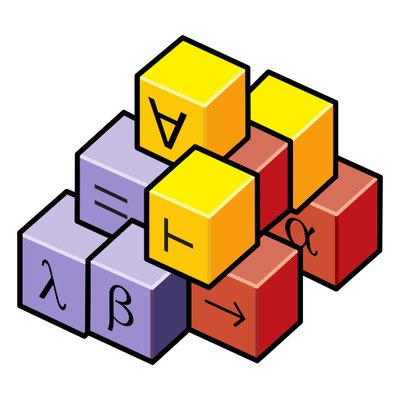
\includegraphics[width=0.3\textwidth]{isabelle.jpg}
}

\only<\downloadisabelle>{
%% \begin{tikzpicture}[remember picture, overlay]
%% \node[anchor=north east] at (current page.north east){
%%     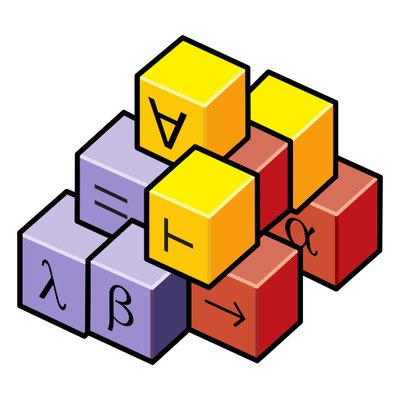
\includegraphics[width=3cm]{isabelle.jpg}
%% };
%% \end{tikzpicture}
  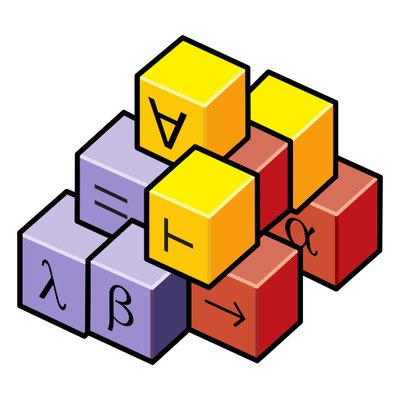
\includegraphics[width=3cm]{isabelle.jpg}
\begin{itemize}
  \item We will use the \href{https://isabelle.in.tum.de/}{\textcolor{red}{Isabelle/HOL}} theorem prover
    \begin{itemize}
    \item Developed by Cambridge, TU Munich, UNSW, and many others
    \end{itemize}
%  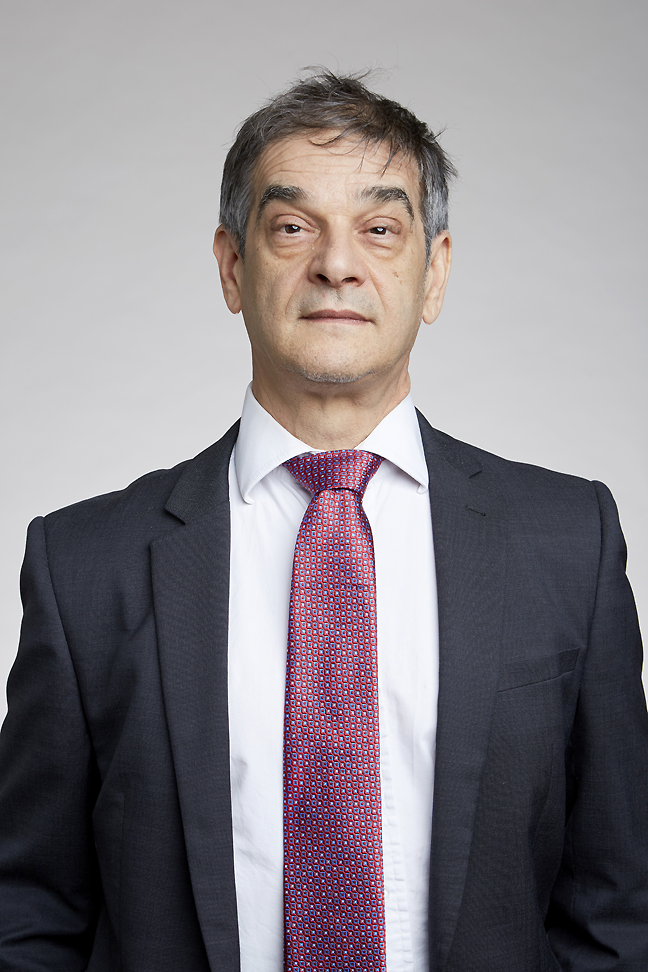
\includegraphics[width=0.15\textwidth]{larry.jpg}
  \item Questions: KEATS+\href{isabelle.zulipchat.com/}{\textcolor{red}{Isabelle's Zulip channel}}
\end{itemize}
}

\note<\books>{
\begin{itemize}
  \item Finally, I would like to note a few relevant points
  \item The first regards books.
  \item I think the best book would be \href{http://www.concrete-semantics.org/}{\textcolor{red}{Concrete Semantics}}, especially the first half of the book.
  \item It gives a good introduction to Isabelle and to functional programming and to proving theorems about those functional programs.
  \item There is also a brief documentation which comes with Isabelle/HOL as you install it, and it is called \href{https://isabelle.in.tum.de/doc/prog-prove.pdf}{\textcolor{red}{Programming and Proving}}.
  \item This will have a lot of information on available proof methods in Isabelle, etc.
\end{itemize}
  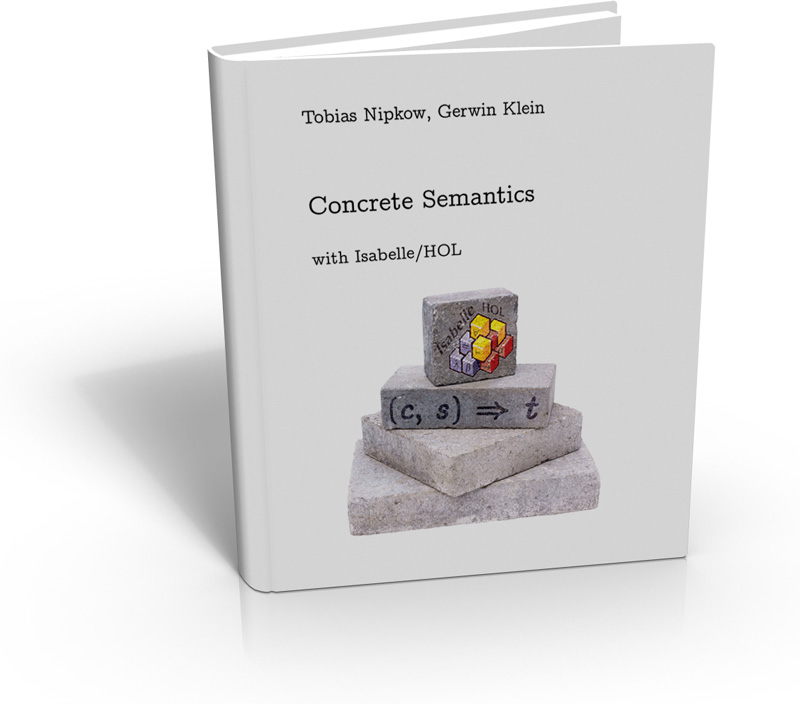
\includegraphics[width=0.5\textwidth]{book.jpg}
}

\only<\books>{
\begin{itemize}
  \item First half of \href{http://www.concrete-semantics.org/}{\textcolor{red}{Concrete Semantics}}
  \item A brief Isabelle/HOL documentation: \href{https://isabelle.in.tum.de/doc/prog-prove.pdf}{\textcolor{red}{Programming and Proving}}
\end{itemize}
  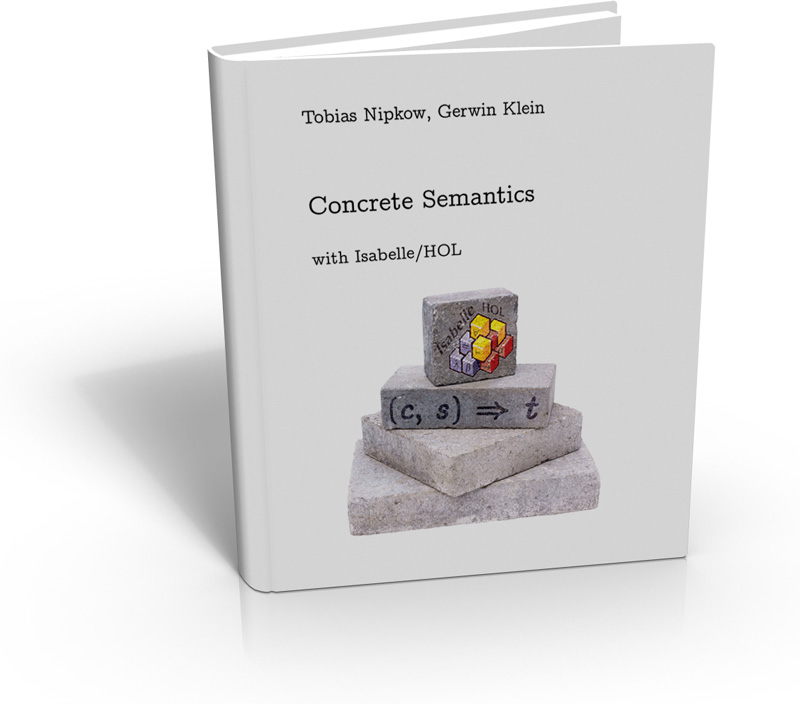
\includegraphics[width=0.5\textwidth]{book.jpg}
}


\note<\assesment>{
\begin{itemize}
\item The assessment of this part will be divided between two things:
  \begin{itemize}
  \item Coursework: this will be an Isabelle assignment, with deadline on 13th December
  \item Exam questions: this will be pen-and-paper proofs of properties of simple functional programs
  \end{itemize}
\end{itemize}
}

\only<\assesment>{
\begin{itemize}
\item Assessment:
  \begin{itemize}
  \item Coursework: an Isabelle assignment, deadline on 13th December
  \item Exam questions: pen-and-paper proofs of properties of a functional program
  \end{itemize}
\end{itemize}
}
\end{frame}

\end{document}
